\documentclass{beamer}
\usepackage{amsmath,amsbsy,amsopn,amstext,amsfonts,amssymb}
\usepackage{isomath}
\usepackage{ulem}
%\linespread{1.6}  % double spaces lines
\usepackage{graphicx}
\usepackage{subfigure}
\usepackage{color}
\usepackage{optidef}  % define optimization problems
\usepackage{multicol}  % multiple columns
\usepackage{listings} % for python code
\usepackage{mathrsfs}

\usepackage{polynom}
\newcommand{\adj}{\mathrm{adj}}
\newcommand{\constrainedmin}[3]{
		\begin{mini*}|s|
		{#2}{#1}{}{}
		\addConstraint{#3}
		\end{mini*}
}

\newcommand{\rwbcomment}[1]{{\color{blue}RWB:#1}}
\newcommand{\defeq}{\stackrel{\triangle}{=}}
\newcommand{\abs}[1]{\left|#1\right|}
\newcommand{\norm}[1]{\left\|#1\right\|}
\newcommand{\iprod}[1]{\left<#1\right>}
\newcommand{\ellbf}{\boldsymbol{\ell}}
\newcommand{\nubf}{\boldsymbol{\nu}}
\newcommand{\mubf}{\boldsymbol{\mu}}
\newcommand{\abf}{\mathbf{a}}
\newcommand{\bbf}{\mathbf{b}}
\newcommand{\cbf}{\mathbf{c}}
\newcommand{\dbf}{\mathbf{d}}
\newcommand{\ebf}{\mathbf{e}}
\newcommand{\fbf}{\mathbf{f}}
\newcommand{\gbf}{\mathbf{g}}
\newcommand{\hbf}{\mathbf{h}}
\newcommand{\ibf}{\mathbf{i}}
\newcommand{\jbf}{\mathbf{j}}
\newcommand{\kbf}{\mathbf{k}}
\newcommand{\lbf}{\mathbf{l}}
\newcommand{\mbf}{\mathbf{m}}
\newcommand{\nbf}{\mathbf{n}}
\newcommand{\obf}{\mathbf{o}}
\newcommand{\pbf}{\mathbf{p}}
\newcommand{\qbf}{\mathbf{q}}
\newcommand{\rbf}{\mathbf{r}}
\newcommand{\sbf}{\mathbf{s}}
\newcommand{\tbf}{\mathbf{t}}
\newcommand{\ubf}{\mathbf{u}}
\newcommand{\vbf}{\mathbf{v}}
\newcommand{\wbf}{\mathbf{w}}
\newcommand{\xbf}{\mathbf{x}}
\newcommand{\ybf}{\mathbf{y}}
\newcommand{\zbf}{\mathbf{z}}
\newcommand{\Jbf}{\mathbf{J}}
\newcommand{\Acal}{\mathcal{A}}
\newcommand{\Bcal}{\mathcal{B}}
\newcommand{\Lcal}{\mathcal{L}}
\newcommand{\Ncal}{\mathcal{N}}
\newcommand{\Rcal}{\mathcal{R}}
\definecolor{darkolivegreen}{rgb}{0.33, 0.42, 0.18}

\makeatletter
\newenvironment<>{proofstart}[1][\proofname]{%
    \par
    \def\insertproofname{#1\@addpunct{.}}%
    \usebeamertemplate{proof begin}#2}
  {\usebeamertemplate{proof end}}
\newenvironment<>{proofcont}{%
  \setbeamertemplate{proof begin}{\begin{block}{}}
    \par
    \usebeamertemplate{proof begin}}
  {\usebeamertemplate{proof end}}
\newenvironment<>{proofend}{%
    \par
    \pushQED{\qed}
    \setbeamertemplate{proof begin}{\begin{block}{}}
    \usebeamertemplate{proof begin}}
  {\popQED\usebeamertemplate{proof end}}
\makeatother

\title{ECEn 671: Mathematics of Signals and Systems}
\author{Randal W. Beard}
\institute{Brigham Young University}
\date{\today}

\begin{document}

%-------------------------------
\begin{frame}
	\titlepage
\end{frame}


%%%%%%%%%%%%%%%%%%%%%%%%%%%%%%%%%%%%%%%%%%%%%%%%%%%%%%%%%%%%%%%%%%
\section{Dual Approximation}
\frame{\sectionpage}

%----------------------------------
\begin{frame}\frametitle{Dual Approximation}
	This section develops an approach that allows approximation in infinite dimensional spaces with finite constraints.
	
	\vfill
	
	For matrices, we will solve the problem
	\begin{mini*}|s|
	{}{\norm{x}}{}{}
	\addConstraint{Ax = b}	
	\end{mini*}
\end{frame}

%----------------------------------
\begin{frame}\frametitle{Dual Approximation, cont.}
\begin{definition}[Affine Space]
	Let $\mathbb{Y}$ be a subspace of $\mathbb{S}$ and let $x_o \in \mathbb{S}$.  The set $\mathbb{V} = x_0 + \mathbb{Y}$ is called a \underline{linear variety} or an \underline{affine} space.
	\begin{center}
	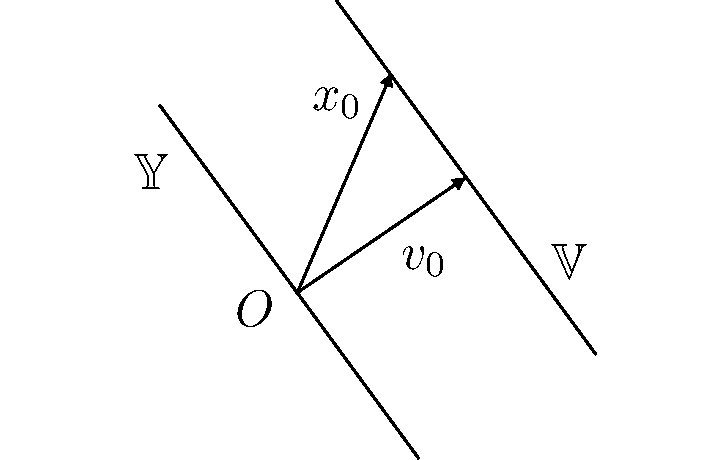
\includegraphics[width=2in]{figures/chap3_affine_space}
	\end{center}
\end{definition}
	
	The projection theorem says that there exists a $v_0 \in \mathbb{V}$ such that
	$v_0 = \underset{v \in \mathbb{V}}{\arg\min}\norm{ v }$ such that
	$v_0 \perp \mathbb{Y}$.

\end{frame}

%----------------------------------
\begin{frame}\frametitle{Dual Approximation, cont.}
	Let $M = span\{y_1, \ldots, y_m\}$ then $\text{dim}(M) < \infty$.
	
	\vfill
	
	If $\text{dim}(\mathbb{S}) = \infty$ then $\text{dim}(M^{\perp}) = \infty$ where $M^{\perp}$ is the set of all $x \in \mathbb{S}$ such that
	\begin{align*}
	\iprod{x, y_1} &= 0 \\
	\vdots \\
	\iprod{x, y_m} &=0	
	\end{align*}
\end{frame}

%----------------------------------
\begin{frame}\frametitle{Dual Approximation, cont.}	

	Now suppose that there are $m$ inner product constraints:
	\begin{align*}
	\iprod{ x, y_1} &= a_1\\
	\vdots\\
	\iprod{ x, y_m} &= a_n
	\end{align*}
	If $\exists x_0$ that satisfies the constraints then so does $x_0 + v$ where $v \in M^{\perp}$ since
	\begin{align*}
	\iprod{ x_0+v, y_j} &= \iprod{ x_0, y_j} + \iprod{v, y_j} \\
						&= \iprod{ x_0,y_j} \\
						&= a_j 
	\end{align*}
	
	Therefore all solutions are in the (infinite dimensional) affine space
	\[ v = x_0 + M^{\perp} \]
	
\end{frame}

%----------------------------------
\begin{frame}\frametitle{Dual Approximation, cont.}	
	\begin{theorem}[Moon Theorem 3.4]
		Let $\{ y_1, \cdots, y_m\} $ be linearly independent in a Hilbert
		space $\mathbb{S}$, and let $M = span\{y_1, \cdots, y_m\}$.	
		The solution of the problem
		\begin{mini*}|s|
		{x\in \mathbb{S}}{\norm{x}^2}{}{}
		\addConstraint{\iprod{x, y_1} &= \alpha_1}	
		\addConstraint{\vdots}
		\addConstraint{\iprod{x, y_m} &= \alpha_m}
		\end{mini*}
		is an element of $M$, i.e., $\hat{x} = \arg\min_{x\in\mathbb{S}}\norm{x}^2 = \sum_{i=1}^{m} c_i y_i$,
		where $\cbf$ satisfies $R\cbf = \boldsymbol{\alpha}$, where $R$ is the Grammian and 
		\[
			\boldsymbol{\alpha} = (\alpha_1, \dots, \alpha_m)^\top.
		\]
	\end{theorem}
	
\end{frame}

%----------------------------------
\begin{frame}\frametitle{Proof:}
	From the previous discussion, the solution lies in the affine space  $\mathbb{V} = x_0 + M^{\perp}$ for some $x_0 \in \mathbb{S}$.
	\begin{center}
	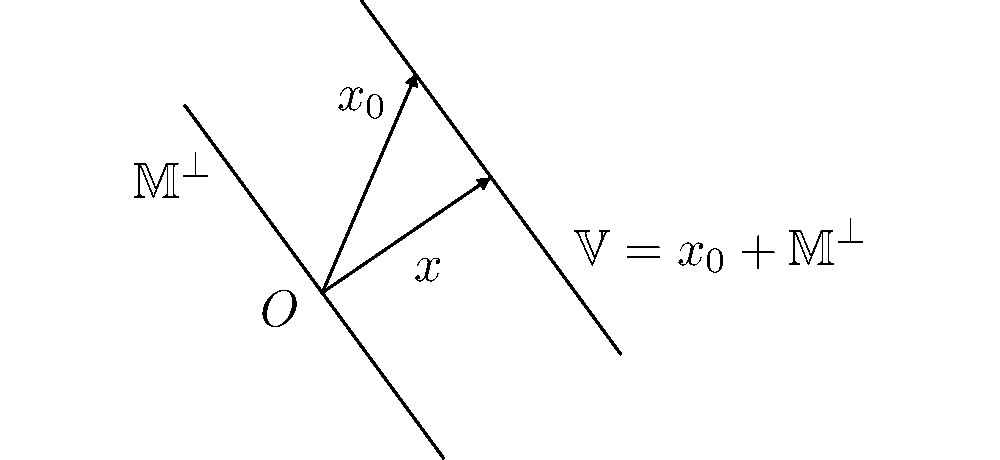
\includegraphics[width=3in]{figures/chap3_dual_approximation}
	\end{center}

	\vfill
	
	The minimum norm solution is orthogonal to $M^{\perp}$ i.e. $\hat{x} \perp
	M^{\perp} \Rightarrow \hat{x} \in M^{\perp \perp} = M$

	\vfill
	
	So $\hat{x}$ is of the form $\hat{x} = \displaystyle \sum_{j=1}^{m}c_jy_j$
\end{frame}

%----------------------------------
\begin{frame}\frametitle{Proof, cont.}
	Now projecting $x$ onto $M$ gives
	\begin{align*}
	\iprod{ \hat{x},y_1} &= \iprod{ \sum c_jy_j, y_1} &= \sum c_j
	\iprod{ y_j, y_1} &= \alpha_1 \\
	\vdots\quad &= \qquad\vdots\qquad &= \qquad\vdots\qquad &= ~~\vdots\\
	\iprod{ \hat{x},y_m} &= \iprod{ \sum c_j y_j, y_m} &= \sum c_j
	\iprod{ y_j,y_m} &= \alpha_m
	\end{align*}
	rewriting in matrix notation gives
	\[ R\cbf = \boldsymbol{\alpha} \]	
\end{frame}


%----------------------------------
\begin{frame}\frametitle{Dual Approximation, Example}
	Given the differential equation
	\[ 
	\ddot{y} + 6\dot{y} + 8y = 4\dot{u} + 10u, \qquad y(0)=\dot{y}(0) =0 
	\]
	Solve the following optimal control problem:
		\begin{mini*}|s|
		{u\in L_2}{\norm{u}^2}{}{}
		\addConstraint{y(1) = 1}	
		\addConstraint{\int_0^1 y(t)dt &= 0}
		\end{mini*}
\end{frame}

%----------------------------------
\begin{frame}\frametitle{Dual Approximation, Example, cont.}
	The corresponding transfer function is
	\begin{align*}
	& H(s) = \frac{4s + 10}{s^2 + 6s + 8} = \frac{1}{s+2} + \frac{3}{s+4} \\
	\Rightarrow & h(t) = e^{-2t} + 3e^{-4t} \\
	\Rightarrow & y(t) = \int_0^t\left[e^{-2(t-\tau)} + 3e^{-4(t-\tau)}\right]u(\tau) d\tau 
	\end{align*}
	
	\vfill
	
	Define the following inner product
	\[ 
	\iprod{f(t), g(t)} = \int_0^1 f(\tau)g(\tau)d\tau 
	\]
	then $y(1) = 1$ can be written as
	\[ \int_0^1 \left[ e^{-2(1-\tau)} + 3e^{-4(1-\tau)}\right]u(\tau)d\tau =
	\iprod{ u,y_1} = 1 \]
	where $y_1(t) = e^{-1(1-t)}+3e^{-4(1-t)}$
\end{frame}

%----------------------------------
\begin{frame}\frametitle{Dual Approximation, Example, cont.}
	The second constraint is of the form 
	\[ \int_0^1 y(t)dt = \int_{t=0}^{t=1} \int_{\tau = 0}^{\tau = t}h(t -
	\tau)u(\tau)d\tau dt = 0 \]
	
	\begin{center}
	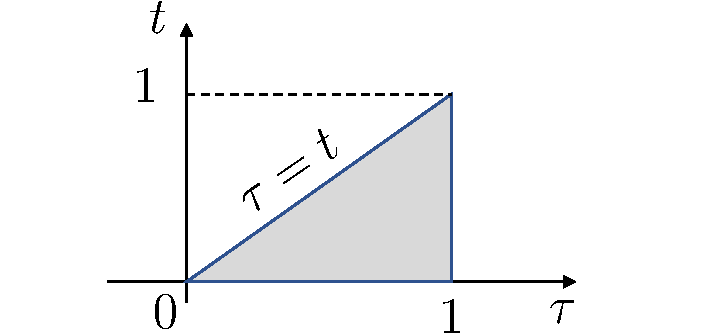
\includegraphics[width=5cm]{figures/chap3_change_of_variables}
	\end{center}
	
	Changing order of integration gives
	\[ = \int_{\tau = 0}^{1}\left[\int_{t = \tau}^{1}
	h(t-\tau)dt\right]u(\tau)d\tau. \]

\end{frame}

%----------------------------------
\begin{frame}\frametitle{Dual Approximation, Example, cont.}	
	Letting $\sigma = t - \tau \Rightarrow t = \sigma + \tau \Rightarrow
	dt = d\sigma$ gives
	\[ = \int_{\tau = 0}^{1} \left[ \int_{\sigma=0}^{\sigma=1-\tau}
	h(\sigma)d\sigma \right] u(\tau) d\tau \]
	\[ = \int_{\tau = 0}^{1}\left( \frac{5}{4} -
	\frac{3}{4}e^{-4(1-\tau)}-\frac{1}{2}e^{-2(1-\tau)}\right)u(\tau)d\tau \]
	\[ = \iprod{u,y_2 } = 0\]
	where 
	\[y_2(t) = \frac{5}{4} -\frac{3}{4}e^{-4(1-\tau)}-\frac{1}{2}e^{-2(1-\tau)} \]
	so we have that 
	\begin{align*}
	\iprod{u,y_1 } &= 1\\
	\iprod{u,y_2 }&= 0
	\end{align*}
	and we want to minimize $\norm{u }^2_{L_2[0,1]}$
\end{frame}
	
%----------------------------------
\begin{frame}\frametitle{Dual Approximation, Example, cont.}	
		
	Let $M = span\{y_1,y_2\}$.

	By Theorem 3.4 
	\[ 
	u \in M \Rightarrow u(t) = c_1y_1(t) + c_2y_2(t) 
	\]
	where
	\[ \left(
	\begin{array}{cc}
	\iprod{y_1,y_1 } & \iprod{y_2,y_1 }\\
	\iprod{y_1,y_2 } & \iprod{y_2,y_2 }
	\end{array}
	\right)\left(
	\begin{array}{c}
	c_1\\
	c_2
	\end{array}
	\right) = \left(
	\begin{array}{c}
	0\\1
	\end{array}
	\right) \]

\end{frame}





\end{document}